\subsection{Physiological signals in frequency- and time-domain}
\label{ch:proc_physio}
All underlying physiological processes are based on the transmission of electrical signals, resulting in a number of electrical measurements in the medical domain, such as EEG or ECG. However, these systems rely on a close contact to the skin in order to measure the electrical signals produced inside the body. Remote sensors have to use a different strategy - the effect that many physiological effects are accompanied by muscle movements that result in temporary changes of posture or volume. Capacitive proximity sensors can be used to measure various physiological parameters that are related to movement of different body parts, including internal organs, most notably the heart. Cheng et al. have presented a system that allows measuring motions and shape changes of body parts using capacitive sensors embedded in garment \cite{cheng2010active}. They were able to detect swallowing and breathing rate. One example for an industrial application is non-contact electrocardiogram (ECG) sensing in cars, intended to detect drowsiness in drivers. Using three electrodes it is possible to detect the heart rate or even acquire a full ECG through various layers of clothing \cite{plessey2012ecg}. MacLachlan presented a system that detects the respiratory rate of a person lying on a bed from a distance of up to 50cm using a single electrode and a highly sensitive sensing method based on spread spectrum methods that are commonly used in wireless communication \cite{MacLachlan2004}.

In this section I present two contributions. The first are approaches to detect the respiratory rate using an analysis in the frequency domain, based on readings by a single capacitive sensor applied close to the chest. The second system uses movement sensing of a person lying in a bed to identify sleep phases.

\subsubsection{Respiratory rate}
\begin{minipage}{\linewidth}
\centering
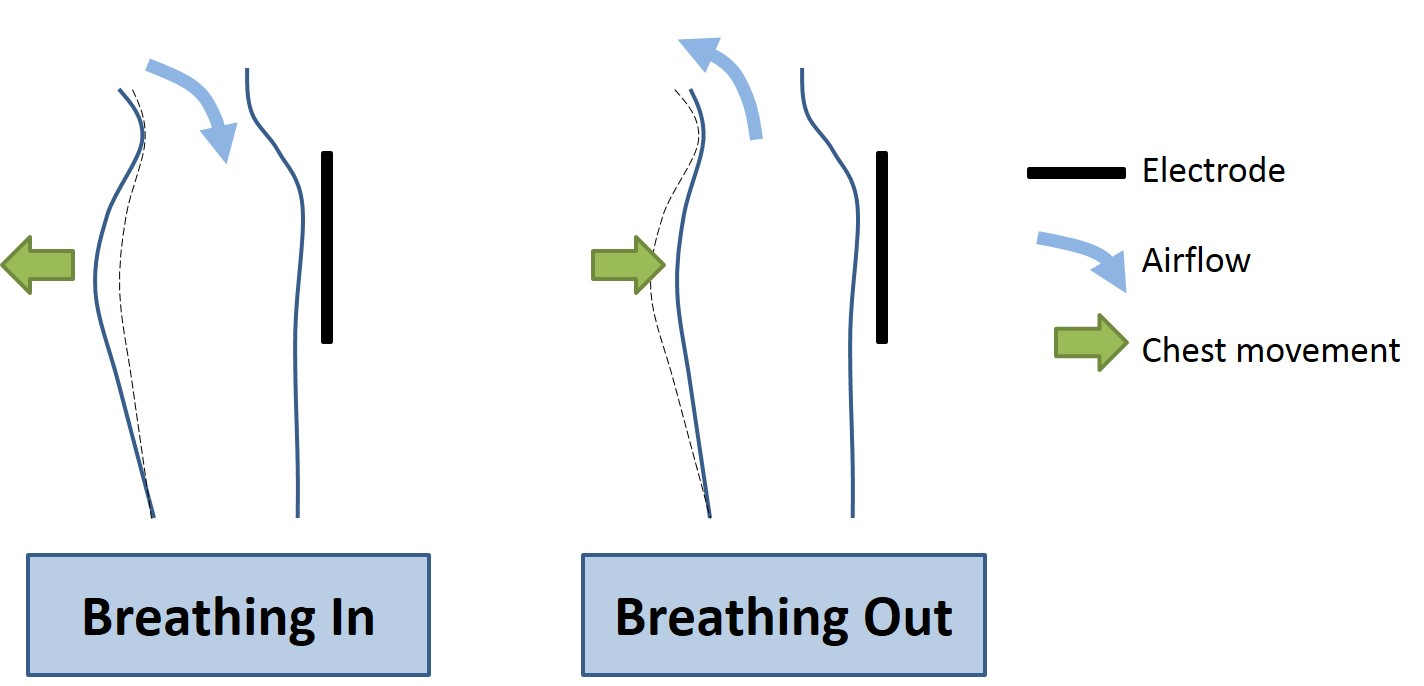
\includegraphics[width=0.8\textwidth]{images/breathing}
\captionof{figure}{Chest movement when breathing in and out}
\label{fig:breathing}
\end{minipage}

The volume changes of the chest while breathing have been a topic of research for a long time \cite{wade1954movements}. If the body of a person is not moving and can be considered at a static distance from a capacitive proximity sensor, the chest movement should translate into a periodically changing sensor value. This system has been developed in cooperation with Sebastian Frank and exemplified using a chair \cite{Braun2013ChairAid}. The breathing rate detection is operating on a single electrode that is placed close to the chest. The basic idea is shown in Figure \ref{fig:breathing}. The surface of the electrode is large, close to the surface and therefore able to pick up the chest movement. Two different methods of data processing are used and fused to get the final breathing rate. Using a fast Fourier transformation the signal is transformed into the frequency space. We are looking for significant signal portions in frequency areas that can be associated to breathing, between $0.1Hz$ and $3Hz$. 

\begin{minipage}{\linewidth}
\centering
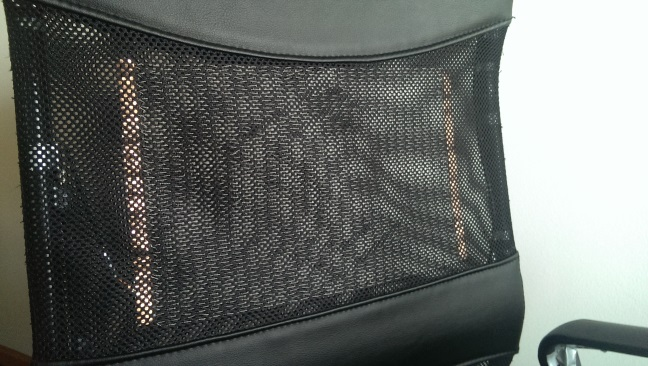
\includegraphics[width=0.8\textwidth]{images/smartchair_thread}
\captionof{figure}{Conductive thread electrode integrated into the backrest of a chair}
\label{fig:smartchair_breathing_curve}
\end{minipage}

The above Figure \ref{fig:smartchair_breathing_curve} shows an example of the sensor data curve generated by the conductive thread sensor behind the back of a person. The chest movement is clearly visible as sinusoidal oscillation of the sensor value. If we have a sufficiently stable baseline the zero-crossings can be calculated. However, as this can't be guaranteed in all cases an adaptive baseline should be used that is reconfigured according to changing states of the sitting person. 

\subsubsection{Sleep phase recognition}
Using movement data to detect sleep phases is an unobtrusive method of sleep monitoring. Studies have shown that the magnitude of movement is typically associated to the following phases in decreasing order: wake, stage 1, REM, stage 2, stage 3 \cite{wilde1983movement}. Another method is distinguishing between awake phase, active sleep and quite sleep and takes into account the order of those phases. This information allows to correlate the actual sleep phases with good certainty \cite{salmi86}. Together with Maxim Djakow and Alexander Marinc I have been working on a system to distinguish sleep phases based on movement data acquired from capacitive proximity sensors \cite{Djakow2013movibed}. 
A typical distribution of sleep phases throughout the night is shown in Figure \ref{fig:proc_phys_sleepphase}. It can be easily seen that the sleep is distributed into different cycles, whereas the sleeping person is moving through the different sleep phases until having a REM phase and then going back to deep sleep. If the only available data is body movements it is becoming more difficult to reliably determine the sleep phase.

\begin{minipage}{\linewidth}
\centering
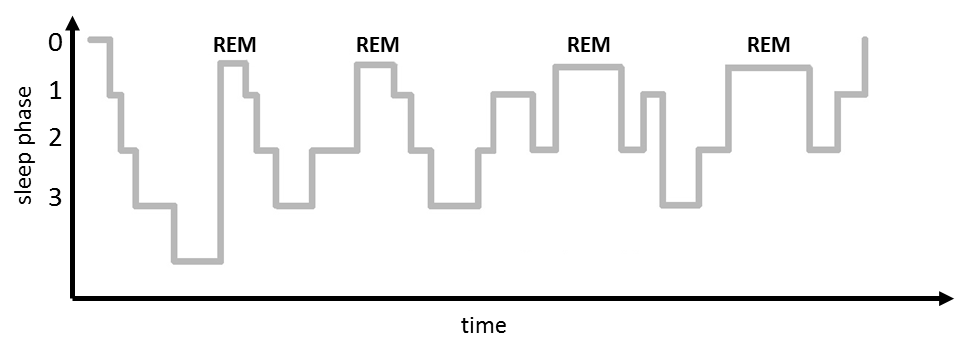
\includegraphics[width=0.6\textwidth]{images/proc_phys_sleepphase}
\captionof{figure}{Example of human sleep phases throughout the night}
\label{fig:proc_phys_sleepphase}
\end{minipage}

The most reliable way to track sleep phases is by using an electroencephalography (EEG); that is measuring the electrical activity of the brain by placing electrodes on the scalp. Various different types of neural oscillations can be distinguished - the most important for sleep phase detection are alpha waves, theta waves, delta waves and sleep spindles. The American Academy of Sleep Medicine (AASM) distinguishes three different phases of non-rapid eye movement sleep (NREM) and REM phase \cite{schulz2008rethinking}. 
\begin{itemize}
\item Stage 1 - occurs mostly in the beginning of sleep. It has slow eye movement, alpha waves disappear and the theta wave appears. 
\item Stage 2 - dreaming is very rare and no eye movement occurs. The sleeper is quite easily awakened. EEG recordings have a tendency for characteristic "sleep spindles"
\item Stage 3 - was previously divided into stages 3 and 4. It is slow-wave sleep (SWS) or deep sleep. Stage 3 used to be the transition between stages 2 and 4 where delta waves began to occur, while delta waves are dominant in stage 4. 
\item REM sleep - is a phase of sleep characterized by random and rapid movement of the eyes. It is considered the lightest phase of sleep and occurs all through the night but gets longer close to morning.
\end{itemize}

Capacitive proximity sensors enable us to detect the presence of suitable object and their relative proximity to the electrode. Consequently a moving object will cause a change of sensor values. If we aggregate these data deviations from an array of sensors we get a reliable measure of objects moving above the electrodes. In the case of our system we can assume that there is a limited number of persons moving on top of the sensors and thus it is possible to associate the sensor values to movement. In the following I will present a suitable method to achieve a reliable detection of the movements of a sleeping person, whereas we are following a similar approach as Salmi and Leinonen \cite{salmi86}.
At any given time t a set of the latest values of all n sensors can be stored as a tuple in the following form: 
\begin{equation}
\overrightarrow{s_t}=\begin{pmatrix}
s_{1_t}\\ 
s_{2_t}\\ 
\vdots \\ 
s_{n_t}
\end{pmatrix}
\end{equation} 

As capacitive proximity sensors are particularly susceptible to external influences, such as temperature, humidity and other electric fields it is necessary to apply filtering on the sensor values. A suitable candidate is a median filter - a low-pass filter method that selects the median object of a sorted set of values, thus discarding outliers and strongly deviating values. This is particularly suited if transmission errors may occur.
If a person is moving on the bed the value of all sensors in detection distance of the moved body parts will change accordingly, the most relevant example in our case being a person moving in its sleep. We can generate a measure of movement intensity by comparing the values at time t with those at time t-1 resulting in:
\begin{equation}
\overrightarrow{d_t}=\left | \overrightarrow{s_t}-\overrightarrow{s_{t-1}} \right | = \begin{pmatrix}
\left | s_{1_t}-s_{1_{t-1}} \right |\\ 
\left | s_{2_t}-s_{2_{t-1}} \right |\\ 
\vdots \\ 
\left | s_{n_t}-s_{n_{t-1}} \right |
\end{pmatrix}
\end{equation}

In subsequent calculations we will use $\overrightarrow{d_t}$ as combined measurement. For distinguishing between wake, active sleep and quiet sleep we are solely interest in the most intense movement. Thus we are testing for the largest value over a set of $m$ samples, generating the value $b_t$.
\begin{equation}
b_t=max(\overrightarrow{d_t1, d_t2, \hdots, d_tm}
\end{equation}

The value $b_t$ is affected by changes in the speed of movement. Therefor as a final step we generate a centered average value of order $2q-1$:
\begin{equation}
\overline{b_t}=\frac{1}{2q-1}\sum_{i=-1}^q{b_{t-i}}
\end{equation}

The resulting value $\overline{b_t}$ allows us to quantify the intensity of movements over a given period. In order to extract an actual body movement from this value we have to quantify a threshold $s(t)$ that is determined by the average of $q$ previous values of $\overline{b_t}$ multiplied with a factor $f$ that has to be evaluated individually for each configuration of bed and sensors. This threshold $s(t)$ allows us to identify a movement $m$ at any time $t$. This behavior is denoted in the following equations:
\begin{equation}
s(t)=\left ( \frac{1}{q}\sum_{i=1}^{q+1}{\overline{b_{t-1}}} \right )\cdot f
\end{equation}
\begin{equation}
m_t=\left\{\begin{matrix}
1,if \; \overline{b_t}> s(t)>\overline{b_{{t-1}}}\\ 
0,else
\end{matrix}\right.
\end{equation}

As previously mentioned it is difficult to determine sleep phases solely by monitoring the movement. Instead following the example of Salmi and Leinonen and distinguish three phases - wake, active sleep and quiet sleep \cite{salmi86}. These are determined by dividing the sleep time into $a$ three-minute epochs $e_{i_a}$ and qualify these as active or quiet by counting the number of movements occurring in those intervals and comparing it to the average amount of movements in all epochs $\overline{e_a}$ determined by the following equations:
\begin{align}
e_{i_a}&=\sum_{e_{i_Start}}^{e_{i_End}}{m_i} & \overline{e_a}&=\frac{1}{n}\sum_{i=0}^n{e_{i_a}}
\end{align}

In consequence we determine the status of any epoch with this final equation:
\begin{equation}
e_{i_a}=\left\{\begin{matrix}
active,if \; e_{i_a}>\overline{e_a}\\ 
quiet,if \; e_{i_a}\leq \overline{e_a}
\end{matrix}\right.
\end{equation}
These active and quiet periods can be semi-autonomously interpreted by humans in order to determine the actual sleep phases. For example initial activity for 20 to 40 minutes followed by a quiet period can be attributed to a person falling asleep. Following quiet phases are a good indicator for deep sleep phases.
 
